% (C)opyright L. Humbert - http://ddi.uni-wuppertal.de/
%
% Um die vorliegende LaTeX-Datei mit pdflatex
% setzen zu können, benötigen Sie 
%
% 0- das LaTeX-Paket pgf (Version 2.xx)
%     http://tug.ctan.org/pkg/pgf
% zum Satz genutzt wurde die aktuelle cvs-Version
% http://www.texample.net/tikz/
%
% 1- http://ddi.uni-wuppertal.de/ddi-wintersemester-2009_2010/ddi-map.sty
%
% 2- das Unterverzeichnis ABB (relativ zum aktuellen Verzeichnis) mit den folgenden Dateien:
%     logo_ponto.pdf, logoddi.pdf, OWL2.pdf, Tuerme.pdf, turmN.pdf, uni_logo.pdf
%     - öffentlich verfügbar unter:
%       http://www.ham.nw.schule.de/pub/bscw.cgi/1077957
%
% 3- die Lizenzdatei (muss in das aktuelle Verzeichnis kopiert werden): 
%     lizenz.xmp
%       https://haspe.homeip.net/projekte/ddi/browser/python/pdflatexLizenz
%      
%
%% Die Vorlage fuer die Veranstaltungskarte/n habe ich von Till Tantau 
%% http://www.tcs.uni-luebeck.de/mitarbeiter/tantau/
%% im März 2008 erhalten.
%% Dank' an Till Tantau für die Bereitstellung der Vorlage.
%%
%% Im Januar 2010 hat Till das Kapitel
%% 6 Tutorial: A Lecture Map for Johannes (S. 67--81)
%% in das Manual eingebaut -- sehr empfehlenswert(!)
%% in Tantau2010, siehe:
%% http://www.texample.net/tikz/builds/
%%
%% Kurzeinführung in die Konstruktion von Wissensnetzen (24. Nov 2008)
%% http://www.statistiker-wg.de/pgf/tutorials/mindmap.htm

%
% Dieses Dokument steht unter der Creative Commons by-nc-sa-Lizenz.
% Folglich darf es beliebig kopiert und bearbeitet werden,
% sofern das Folgeprodukt wiederum unter dieser Lizenz vertrieben wird.
% Eine kommerzielle Nutzung ist nicht erlaubt.
%
% Die detaillierten Lizenzbedingungen finden sich auf der Seite
% http://creativecommons.org/licenses/by-nc-sa/3.0/deed.de
%
%
% Der Inhalt des vorliegenden Dokuments unterliegt der
% creativecommons.org/licenses/by-nc-sa/3.0/deed.de-Lizenz
%
% Kurz zusammengefasst, bedeuten die Bedingungen in lesbarer Form:
%
% Sie dürfen das Werk vervielfältigen, verbreiten und "offentlich
% zugänglich machen
%
% Bearbeitungen des Werkes anfertigen
%
% Dabei müssen Sie die folgenden Bedingungen beachten
% by -- Namensnennung
% nc -- Keine kommerzielle Nutzung
% sa -- Weitergabe unter gleichen Bedingungen
%
% Die oben beschriebene Lizenz findet sich in maschinenlesbarer Form unter
% https://haspe.homeip.net/projekte/ddi/browser/python/pdflatexLizenz
% (lizenz.xmp).
%
% Im Falle einer Verbreitung müssen Sie anderen die Lizenzbedingungen,
% unter die dieses Werk fällt, mitteilen. Am Einfachsten ist es, einen
% Verweis auf die oben angegebene Seite einzubinden.
% Jede der vorgenannten Bedingungen kann aufgehoben werden, sofern Sie die
% Einwilligung des Rechteinhabers dazu erhalten.
% Diese Lizenz lässt die Urheberpers"onlichkeitsrechte unberührt.
%
% Details dazu, wie eine maschinenlesbare Lizenzdatei in das Dokument 
% eingebunden werden kann, finden sich in der Fachseminarzeitung:
% http://humbert.in.hagen.de/rhinodidactics/Artikel/latex-2007-10-01.html 
%
%
%
\documentclass[german,landscape]{article}
\usepackage[utf8]{inputenc}

\title{Didaktik der Informatik}
\author{Prof. Dr. Ludger Humbert}

\usepackage{amsmath}
\usepackage{ddi-map}
\usepackage[T1]{fontenc}
% Einbinden der Lizenz (fuer das PDF-Dokument) durch pdflatex
\usepackage{xmpincl}
\includexmp{lizenz}

\hypersetup{%
    pdftitle={Veranstaltungskarte – Didaktik der Informatik – Sommersemester 2010 und Wintersemester 2010/2011 – \jobname },
    pdfsubject={\jobname},
    pdfauthor={Prof. Dr. L. Humbert – humbert at uni-wuppertal dot de  – http://ddi.uni-wuppertal.de/ – CC-Lizenz: http://creativecommons.org/licenses/by-nc-sa/3.0/deed.de},
    pdfkeywords={Veranstaltungskarte,Informatikunterricht,Didaktik,Modulkonzept,Mobiltelefon,S60,Python,Informatik,allgemeine Bildung,Paradigmen,Freihandversuche}
}

\usetikzlibrary{fadings,shadows}

% The lecture information
%\tikzstyle{lecture annotation}=[lecture annotation white,/ddia/urlprefix/.add={}{ddi-sommersemester-2010}]
%
\tikzset{every concept/.style={circular drop shadow}}

\tikzstyle{teaching informatics}=[concept color=teaching informatics,set style={{fade}=[concept color=teaching informatics!60]}]
\tikzstyle{informatics}=[concept color=informatics,set style={{fade}=[concept color=informatics!60]}]
\tikzstyle{pedagogy}=[concept color=pedagogy,set style={{fade}=[concept color=pedagogy!60]}]
\tikzstyle{schulinformatik}=[concept color=schulinformatik,set style={{fade}=[concept color=schulinformatik!60]}]

% Colors
\colorlet{lecture}{orange}

\colorlet{schulinformatik}{blue}
\colorlet{teaching informatics}{orange}
\colorlet{informatics}{green!50!black}
\colorlet{pedagogy}{red}

\colorlet{schulinformatik.bg}{schulinformatik!35}
\colorlet{teaching informatics.bg}{teaching informatics!35}
\colorlet{informatics.bg}{informatics!35}
\colorlet{pedagogy.bg}{pedagogy!35}

\definecolor{medium}{rgb}{.5,.5,.51}
\definecolor{calendar.bg}{rgb}{.7,.7,.71}
\definecolor{black75}{rgb}{.25,.25,.26}
\definecolor{black20}{rgb}{.8,.8,.81}

\listfiles % damit in der Log-Datei alle Pakete und benoetigten Dateien stehen

\begin{document}
 \begin{map}
 
  \begin{scope}[a0 mindmap]

   \tikzstyle{level 1}+=[level distance=25cm]
   \tikzstyle{level 2}+=[level distance=11cm]
   \tikzstyle{level 3}+=[level distance=9.3cm]

   \node[concept,fill=white,text=black,line width=1ex] (ddi) 
    [xshift=-0.05\picturewidth,yshift=-.0357\pictureheight]
    {
     \href{http://ddi.uni-wuppertal.de/}{\uppercase{Didaktik der Informatik}}
    }

   child [grow=-148,pedagogy] { node [concept] (pedagogy) {Lehren und Lernen}
    [clockwise from=-30]
    child { node[concept] (edu science)    {Erziehungs\-wissenschaft} 
       [clockwise from=10]
       child { node[concept] (education)     {Bildung}}
       child { node[concept] (society)       {Gesellschaft}}
       child { node[concept] (functions of school){Funktionen der Schule}
         [counterclockwise from=240]
         child { node[concept] (qualification)    {Qualifikation}           }
         child { node[concept] (allocation)       {Allokation Selektion}    }
         child { node[concept] (socialisation)    {Sozialisation Integration Legitimation} }
       }
    }    
    child       { node[concept] (learn theory)   {Lerntheorie} 
       [counterclockwise from=270]
       child { node[concept] (behaviorism)       {Behaviorismus}    }
       child { node[concept] (cognitivism)       {Kognitivismus}    }
       child { node[concept] (constructivism)    {Konstruk\-tivis\-mus} }
    }
    child { node[concept] (teaching) {Lehren}
       [clockwise from=295]
       child       { node[concept] (formal stages)        {Formalstufen}           }
       child       { node[concept] (instruction problems) {Probleme der Instruktion}
          [clockwise from=-80]
          child { node[concept] (instruction theory)  {Theorie?}  }
          child { node[concept] (empirie)             {Empirie}   }
          child { node[concept] (practical)           {Praktisch} }
       }
       child       { node[concept] (phases)         {Phasen}               }
       child       { node[concept] (triangle)       {Didaktisches Dreieck} }
       child       { node[concept] (plan models)    {Planungs\-modelle}
          child [grow=45] { node[concept] (systemtheoretical) {System\-theorie}      }
          child [grow=90] { node[concept] (berlin)  {Berliner/""Hamburger\\Modell}   }
          child [grow=145]{ node[concept] (klafki)  {Kritisch-konstruktive Didaktik} }
       }
    }
    child { node[concept] (competencies) {Lernziele und Kompetenzen}
       [counterclockwise from=30]
       child  { node[concept] (input)              {Input} }
       child  { node[concept] (output)            {Output} }
       child  { node[concept] (competence)     {Kompetenz} }
       child  { node[concept] (operator)        {Operator} }
       child  { node[concept] (taxonomy)       {Taxonomie}
          [counterclockwise from=180]
          child  { node[concept] (bloom)         {Bloom}
            [clockwise from=100]
            child  { node[concept] (kognitiv)         {kognitiv}         }
            child  { node[concept] (affektiv)         {affektiv}         }
            child  { node[concept] (psychomotorisch)  {psycho\-motorisch}}
         }
       }
    }
  }
  child [grow=148,teaching informatics] { node[concept] (teaching informatics) {Informatik\-unterricht}
     [counterclockwise from=-5]
     child { node[concept] (forms) {Form}
        [counterclockwise from=-3]
        child { node[concept] (inner) {innere}
           [counterclockwise from=-20]
           child { node[concept] (problemoriented) {Problem\-orientiert} }
           child { node[concept] (projectoriented) {Projekt\-orientiert} }
        }   
        child [grow=50] { node[concept] (external) {äußere}
           [clockwise from=-5]
           child { node[concept] (compulsory) {Pflicht\-unterricht} }
           child { node[concept] (elective)   {Wahlfach}            }
        }
     }
     child { node[concept] (planning cs) {Planung}
        [counterclockwise from=15]
        child { node[concept] (approaches) {Vorgehens\-weisen}
          [counterclockwise from=0]
          child { node[concept] (ppl) {A Pedagogical Pattern Language}       }
          child { node[concept] (upp) {Unterrichts\-planung pro\-fessionell} }
        }
        child { node[concept] (dimensions) {Dimensionen}
          [counterclockwise from=50]
          child { node[concept] (goals) {Ziele} 
            [counterclockwise from=-10]
            child { node[concept] (curricula)        {Lehr\-pläne}         }
            child { node[concept] (framework)        {Rahmen\-vorgaben}    }
            child { node[concept] (subject to teach) {fachliche Inhalte}   }
          }
          child { node[concept] (phases)       {Phasen}         }
          child { node[concept] (methods)      {Methoden}       }
          child { node[concept] (aux resource) {(Hilfs-)Mittel} 
            [counterclockwise from=70]
            child { node[concept] (worksheets) {Arbeits\-blätter}                   }
            child { node[concept] (foils)      {Overhead-Folien}                    }
            child { node[concept] (ifsystems)  {Informatik\-systeme \\ \href{http://www.ham.nw.schule.de/pub/bscw.cgi/114759}{\Mobilefone} }}
            child { node[concept] (white board){White-Board\\Tafel}                 }
          }
        }  
     }
     child { node[concept] (concepts) {Konzepte}
        [counterclockwise from=75]
        child { node[concept] (oos) {Objekt\-orientierte Sicht} 
            child [grow=90] { node[concept] (ponto){ \href{http://ham.nw.schule.de/pub/bscw.cgi/73468}{
\includegraphics[scale=0.8]{ABB/logo_ponto.pdf}}} }
            child [grow=-15] { node[concept] (sum)  {Klassen\-biblio\-thek Stifte und Mäuse}                         }
        }
        child { node[concept] (fs) {Funktionale Sicht} 
            [counterclockwise from=90]
            child  { node[concept] (tk)    {Tabellen\-kalkulation}           }
            child  { node[concept] (logo)  {Model\-lierung Umsetzung mit Logo} }
        }
        child { node[concept] (ws) {Wissensbasierte Sicht} 
            [counterclockwise from=120]
            child  { node[concept] (erdb) {ER-Modellierung Datenbank} }
            child  { node[concept] (pm)   {Prädikative Modellierung}  }
        }
        child { node[concept] (ps) {Phänomene der Informatik} 
            [counterclockwise from=145]
            child  { node[concept] (everyday) {Alltag}    }
            child  { node[concept] (design)   {Gestalten} }
        }
        child { node[concept] (hs) {Geschichtliche Aspekte} 
            [counterclockwise from=170]
            child  { node[concept] (abstr) {Abstraktions\-stufen}       }
            child  { node[concept] (conc)  {Kon\-zept\-ent\-wick\-lung} }
        }
        child { node[concept] (pw) {>>Spiel<<\-welten} }
     }
     child [grow=193] { node[concept] (gender) {Gender} 
        [counterclockwise from=170]
        child { node[concept] (te) {Terminologie}           }
        child { node[concept] (qlv) {qualitativ}            }
        child [grow=330]{ node[concept] (qtv) {quantitativ} }
     }
  }
  child [grow=32,informatics] { node[concept] (informatics) {Informatik}
    [clockwise from=120]
    child { node[concept] (theoretical informatics)  {Theoretische Informatik}
      [counterclockwise from=100]
      child[fade] { node[concept] (type theory)         {Typtheorie}              }
      child[fade] { node[concept] (machine models)      {Maschinen\-modelle}      }
      child[fade] { node[concept] (ai)                  {Künstliche Intelligenz}  }
      child { node[concept] (automata theory)           {Automaten\-theorie}      }
      child { node[concept] (formal languages)       {Theorie\\formaler Sprachen} }
      child { node[concept] (complexity theory)      {Komplexitäts\-theorie}      }
    }
    child { node[concept] (practical cs)     {Praktische Informatik}
      [clockwise from=90]
      child { node[concept] (algorithms)          {Algo\-rithmen}
        [counterclockwise from=85]
        child       { node[concept] (graph algorithms)     {Graph\-algorithmen}         }
        child[fade] { node[concept] (geometric algorithms) {geo\-metrische}             }
        child       { node[concept] (algorithmic methods)  {algorith\-mische Methoden}  }
        child 		{ node[concept] (sorting)              {Sortieren}     		}
        child 		{ node[concept] (searching)            {Suchen}        		}
        child 		{ node[concept] (optimization)         {Opti\-mierung} 		}
      }
      child { node[concept] (data structures)     {Daten\-strukturen}
        [clockwise from=90]
        child { node[concept] (structured data structures) {zusammen\-gesetzte} 	}
        child { node[concept] (simple data structures) {einfache}			}
      }
      child { node[concept] (software engineering) {Software\-technik}
        [clockwise from=60]
        child       { node[concept] (modeling)     {Model\-lierung} 
          [clockwise from=30]
          child       { node[concept] (oom)     {Objekt\-orientiert}
            [clockwise from=30]
            child  { node[concept] (ooa)     {Analyse OOA}            }
            child  { node[concept] (ood)     {Gestal\-tung OOD}       }
            child  { node[concept] (oop)     {Implemen\-tierung\\OOP} }
          }
        }
        child       { node[concept] (structuring)  {Struktu\-rierung}  }
        child       { node[concept] (modulization) {Modulari\-sierung} }
        child       { node[concept] (planning)     {Planung} 
          [clockwise from=30]
          child {node[concept] (waterfall) {Wasserfall}          }
          child {node[concept] (steps)     {STEPS} 		 }
          child {node[concept] (xp)        {eXtreme Programming} }
        }
      }
      child { node[concept] (programming languages) {Pro\-grammier\-sprachen}
      }
    }
    child { node[concept] (applied cs) {Angewandte Informatik}
      [clockwise from=30]
      child { node[concept] (databases) {Daten\-banken}       }
      child { node[concept] (os) {Betriebs\-systeme}          }
      child { node[concept] (applications) {Anwendung}        }
    }
    child { node[concept] (technical informatics) {Technische Informatik}
      [clockwise from=15]
      child       { node[concept] (processors) {Prozessoren}    }
      child[fade] { node[concept] (circuits)   {Schalt\-kreise} }
      child       { node[concept] (periphery)  {Peripherie}     }
      child       { node[concept] (networks)   {Netzwerke}      }
      child[fade] { node[concept] (robotics)   {Robotik}        }
    }
    child { node[concept] (informatics and society) {Informatik und Gesellschaft}
    }
  }
  child [grow=-42,schulinformatik] { node[concept] (schulinformatik) {Schul\-informatik}
    [clockwise from=10]
    child { node[concept] (didactical recommendations) {Fachdidaktische Empfehlungen -- Konzepte}
      [clockwise from=30]
      child { node[concept] (towers of informatics) {Informatiktürme} 
        child [grow=15]{ node[concept] (informatics tower n) {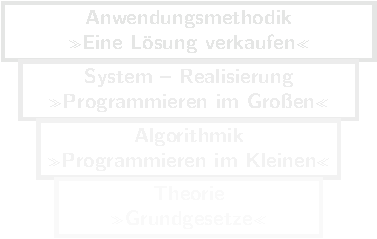
\includegraphics[scale=0.47]{ABB/turmN.pdf}} }
        child [grow=60]{ node[concept] (informatics tower f) {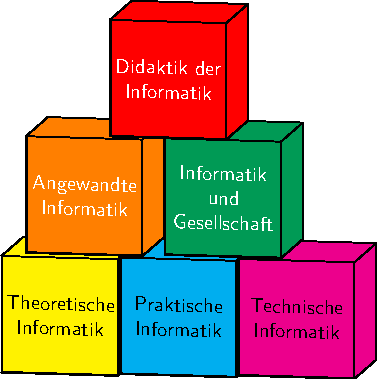
\includegraphics[scale=0.47]{ABB/Tuerme.pdf}} 				  }
      }
      child { node[concept] (modular concept)       {Modulkonzept}                      }
      child { node[concept] (information based)     {Informations\-orientierter Ansatz} }
      child { node[concept] (fundamental ideas)     {Fundamentale Ideen}                }
      }
    child { node[concept] (didactical orientation) {\ldots{}orientierungen über die Zeit}
      [clockwise from=-15]
      child { node[concept] (society oriented)     {Gesellschafts-} }
      child { node[concept] (application oriented) {Anwendungs-}    }
      child { node[concept] (user oriented)        {Benutzungs-}    }
      child { node[concept] (algorithm oriented)   {Algorithmen-}   }
      child { node[concept] (computer oriented)    {Rechner-}       }
      }
    child { node[concept] (institutionalisation) {Institutionalisierung}
      [counterclockwise from=180]
      % den Verweis regelmaessig pruefen ...
      child { node[concept] (examination) { \href{http://is.gd/fPjn5}{EPA 2004} } }
      child { node[concept] (teacher training) {Infor\-matik\-lehrer\-aus\-bil\-dung 1975} 			}
      child { node[concept] (first attempts)  {Schulversuche 1969}						}
      }
    child { node[concept] (bildungsstandards) { \href{http://is.gd/fPjpW}{Bildungs\-standards Informatik}}
      }
  };
  %
  \begin{scope}[concept color=medium,level 2 concept,font=\scshape]
    % The extra topics
    \node [concept] (ee)                     at ([shift=(right:22.8)  ]technical informatics) {Elektro\-technik};
    \node [concept] (linguistics)            at ([shift=(   up:23)    ]formal languages) {Linguistik};
    \node [concept] (mathematics)            at ([shift=(   up:18)    ]theoretical informatics) {Mathematik};
    \node [concept] (economy)                at ([shift=(right:18.1)  ]applied cs)             {Wirtschaft};
    \node [concept] (philosophy)             at ([shift=(north east:6.2) ]education) {
\includegraphics[scale=0.6]{ABB/OWL2.pdf}};
  \end{scope}
 \end{scope}


  \begin{lecture title}
    \href{http://ddi.uni-wuppertal.de/index-wintersemester_2010-2011.html}{Didaktik der Informatik 2010--2011}
  \end{lecture title}

  \begin{lecture learning targets}
      \item Grundlegende pädagogische, didaktische und fachdidaktische Positionen für den Informatikunterricht beschreiben und einordnen 
      \item Allgemeinbildende Elemente der Informatik kennen, einordnen, prüfen und vorausschauend planen (inkl. Unterrichtssequenzen/-reihen)
      \item Problemorientierten Informatikunterricht kennen und beispielhaft illustrieren 
      \item Qualitätskriterien für guten Informatikunterricht angeben
      \item Möglichkeiten und Grenzen der lerngruppenangemessenen Umsetzung grundlegender Erkenntnisse der Informatikdidaktik begründet einschätzen
  \end{lecture learning targets}

  % Graphics
  \begin{scope}[black20,thick]
    \node [below=2ex] at (economy)
    {\huge \EURdig};

    \node [below=2ex] at (mathematics)
    {$\sum_{i=1}^\infty \frac{1}{n^2}=\frac{\pi^2}{6}$};

    \path [font=\tiny,level distance=2.5ex,sibling distance=3.5ex,inner sep=1pt]
    node [below=2ex,xshift=1ex] at (linguistics)
    {Satz}
    child { node {\strut Subjekt}
      child { node {Das} }
      child { node {Sein} }
    }
    child { node{\strut ist.} };

    \node [draw,circle,minimum size=7mm,below=4ex] (transistor) at (ee) {};
    \draw ([xshift=-2mm]transistor.west) -- +(4mm,0pt) coordinate (transistor-mid);
    \draw[very thick] (transistor-mid) +(0mm,2mm) -- +(0mm,-2mm);
    \draw (transistor-mid) -- +(4mm,4mm);
    \draw[-stealth] (transistor-mid) -- +(2mm,-2mm);
    \draw (transistor-mid) -- +(4mm,-4mm);
  % 
  \end{scope}
  
  % The backgrounds
  \begin{pgfonlayer}{background}
    % The four quadrants
    \fill[informatics.bg]          (ddi) rectangle (current bounding box.north east);
    \fill[schulinformatik.bg]      (ddi) rectangle (current bounding box.south east);
    \fill[pedagogy.bg]             (ddi) rectangle (current bounding box.south west);
    \fill[teaching informatics.bg] (ddi) rectangle (current bounding box.north west);

    % Shadings between quadrants
    \shade[left color=teaching informatics.bg,right color=informatics.bg]
      (ddi.135) rectangle (ddi.45 |- current bounding box.north east);
    \shade[top  color=informatics.bg,bottom color=schulinformatik.bg]
      (ddi.45)  rectangle (ddi.-45 -| current bounding box.north east);
    \shade[left color=pedagogy.bg,right color=schulinformatik.bg]
      (ddi.-45) rectangle (ddi.-135 |- current bounding box.south west);
    \shade[top color=teaching informatics.bg,bottom color=pedagogy.bg]
      (ddi.135) rectangle (ddi.-135 -| current bounding box.south west);

    % Calendars: durch Knoten in der N"ahe der Kalenderdaten k"onnen die 
    %            Farbverl"aufe gegen"uber dem Kalender justiert werden
    % daher sind verschiedene Versuche n"otig, um die Einstellungen
    % zu optimieren.
    \fill[calendar.bg] (-.5\picturewidth,-.5\pictureheight) rectangle +(.1\picturewidth,\pictureheight);
    \shade[left color=calendar.bg,right color=pedagogy.bg,shift=(empirie.south west),xshift=-1.5cm,yshift=-0.019\pictureheight-3cm]
       (-0.04\picturewidth,0pt) rectangle (-0.067\picturewidth,.56\pictureheight);
    \shade[left color=calendar.bg,right color=teaching informatics.bg,shift=(taxonomy.north west),xshift=1cm,yshift=-1.5cm]
       (-0.084\picturewidth,0pt) rectangle (0cm,.75\pictureheight);
    \fill[calendar.bg] (.5\picturewidth,-.5\pictureheight) rectangle +(-.1\picturewidth,\pictureheight);
    \shade[right color=calendar.bg,left color=informatics.bg,shift=(ee)]
       (0.034\picturewidth,0pt) rectangle (0cm,.75\pictureheight);
    \shade[right color=calendar.bg,left color=schulinformatik.bg,shift=(ee)]
       (0.034\picturewidth,0pt) rectangle (0cm,-.75\pictureheight);


    % The connections
    \begin{scope}[line width=1mm,shorten <=2mm,shorten >=2mm,cap=round,draw=medium]
     \draw [concept connection]
            (linguistics)             edge (formal languages)
            (mathematics)             edge (theoretical informatics)
            (formal languages)        edge (automata theory)
            (automata theory)         edge (complexity theory)
            (formal languages)        edge (complexity theory)
            (ai.-135)                 edge[bend right] (robotics.135)
            (technical informatics)   edge (ee)
            %
            (economy)                 edge (technical informatics)
            (economy)                 edge (software engineering)
            (economy)                 edge (applied cs)
            (informatics and society) edge (society)
            %%
            %%% -- Zuordnung der -orientierungen zu den Fachgebieten der Informatik --
            (algorithm oriented)    edge  (practical cs)
            (computer oriented.90)     edge[bend left]  (technical informatics)
            (application oriented)  edge [bend left=-90] (applied cs)
            (user oriented)         edge (software engineering)
            (society oriented)      edge [bend left]  (society.135)
            %%%
            % Informatiktuerme ...
            (informatics tower n)   edge [bend right] (informatics)
            (informatics tower f)   edge [bend right] (informatics)
            % konzeptionelle Ansaetze
            %
            (modular concept)       edge [bend left]  (practical cs)  
            (modular concept)       edge   (constructivism)		
            (modular concept)       edge [bend left]  (theoretical informatics)
            (information based)     edge [bend left=-50] (applied cs)
            (fundamental ideas)     edge   (cognitivism)		
            %%
            (institutionalisation)  edge[bend right] (society.35)
            (databases)             edge             (applications)
            %% Wintersemester -- Anpassung Verbindungen
            (concepts)              edge (modeling)
            (oos)                   edge (oom.20) 
            ;
    \end{scope}
  \end{pgfonlayer}

  
  \begin{calendar left}
   % Sommersemester -- Kalender
%% Karfreitag:       2.04.2010
%% Ostermontag:      5.04.2010
%%--------------------------------------------------
    \calendar [dates=2010-04-12 to 2010-07-last]
%% Vorlesungszeitraum: Montag, 12.04.2010 -- Freitag, 23.07.2010
%% Tag der Arbeit:  Samstag,     1.05.2010 +
%% Himmelfahrt:     Donnerstag, 13.05.2010 +
%% Pfingstmontag:   Montag,     24.05.2010 +
%% Fronleichnam:    Donnerstag,  3.06.2010 +
       if (equals=05-01,equals=05-13,equals=05-24,equals=06-03) [holiday]
%% Pfingstenferien Vorlesungsende: Freitag, 22.05.2010  Vorlesungsbeginn: Montag, 31.05.2010
       if (between=2010-05-22 and 2010-05-31) [white]
       if (between=2010-04-14 and 2010-07-24) {} else [holiday];

  \annotatedrangestart{2010-04-15}{Gender -- Informatik Geschichte  -- Einführung}
  \annotatedrangestart{2010-05-06}{Schulinformatik --  Standards -- Entwicklungslinien -- Lernen}
  \annotatedrangestart{2010-06-17}{Informatikunterricht -- Planung  -- Arbeitsweisen}
  \annotatedrangestart{2010-07-08}{Moral -- Ethik -- Profession-- Leistung -- Beispiele}
  
    \annotation[title=Organisatorisches -- Einführung,number=A1,%
                ddi a lecture,%
                above,at=(ddi.north),%
                url=ddi-sommersemester-2010/Sommersemester_2010-DdI-1.pdf,%
                date=2010-04-15]
    {
     \item Begriffe Didaktik und Methodik kennen
     \item Ziele der Fachdidaktik Informatik als Bildungsziele einordnen
     \item Wissenschaftstheoretische Einordnung der Informatik 
    };
    \annotation[title=Informatik -- geschichtliche Aspekte,number=A2,%
                ddi a lecture,%
                right,at=(ddi.east),%
                url=ddi-sommersemester-2010/Sommersemester_2010-DdI-2.pdf,%
                date=2010-04-22]
    {
     \item Alleinstellungsmerkmale der Informatik im Zusammenhang der geschichtlichen Entwicklung herausarbeiten
     \item Entwicklung und Herausbildung der Wissenschaft Informatik im Kontext darstellen
     \item Konsequenzen der Abgrenzungsproblematik erläutern -- Transdisziplinarität versus Interdisziplinarität
     \item \frqq{}Fundamentals\flqq{} der Fachwissenschaft begründen
    };
    \annotation[title=Genderdiskussion,number=A3,%
                ddi a lecture,%
                above,at=(gender.west),%
                url=ddi-sommersemester-2010/Sommersemester_2010-DdI-3.pdf,%
                date=2010-04-29]
    {
     \item Begriffe, Diskussionskontext und Ergebnisse verdeutlichen
     \item Statistische Daten kennen
     \item Vorschläge zur Beeinflussung der Situation bewerten 
     \item Eigenes Handeln auf dem Hintergrund der Ergebnisse reflektieren
    };
    \annotation[title=Grundfragen des Lernens,number=A4,%
                ddi a lecture,%
                left,at=(pedagogy.west),%
                url=ddi-sommersemester-2010/Sommersemester_2010-DdI-4.pdf,%
                date=2010-05-06]
    {
     \item Lerntheoretische Grundlagen und Didaktische Grundorientierungen im Zusammenhang darstellen
     \item Unterrichtskonzepte als Prinzipien methodischen Handelns kennen
     \item Erkenntnisse der Lerntheorie anwenden
     \item Fachdidaktische Basiskonzepte benennen und einordnen
    };
    \annotation[title=Entwicklungslinien der Schulinformatik,number=A5,%
                ddi a lecture,%
                above,at=(schulinformatik.north),%
                url=ddi-sommersemester-2010/Sommersemester_2010-DdI-5.pdf,%
                date=2010-05-20]
    {
     \item Ziele der Informatischen Allgemeinbildung begründen können
     \item Zugänge zur Informatischen Allgemeinbildung kennen
     \item Konzepte der Informatikbildung über die Zeit einordnen
     \item Informatiktürme zur Darstellung der Struktur des Faches kennen
    };
    \annotation[title=Schulinformatik -- Normierung,number=A6,%
                ddi a lecture,%
                right,at=(bildungsstandards.south),%
                url=ddi-sommersemester-2010/Sommersemester_2010-DdI-6.pdf,%
                date=2010-06-10]
    {
     \item Wandel von der Input- zur Outputorientierung erklären und einordnen
     \item Wissenschaftliche Einordnung der Qualität von Testverfahren für Kompetenzen vornehmen
     \item Funktion(en) der Notengebung an Beispielen darstellen und Widersprüche herausarbeiten
     \item Stellenwert der Bildungsstandards Informatik, der EPA und des Zentralabiturs kennen und darstellen
    };
    \annotation[title=Besondere Arbeitsweisen,number=A7,%
                ddi a lecture,%
                right,at=(forms.north east),%
                url=ddi-sommersemester-2010/Sommersemester_2010-DdI-7.pdf,%
                date=2010-06-17]
    {
     \item Einsatz von Informatikmitteln im Informatikunterricht einordnen
     \item Fachliche sowie fachdidaktische Sicht auf Problemlösen und Projekt(e) vorstellen
     \item Formen und Ausprägung der Differenzierungen benennen und bezüglich der Informatik einordnen
     \item Mindestens drei Formen der inneren Differenzierungsmöglichkeiten kennen und vorbereiten
    };
    \annotation[title=Informatikunterrichtsplanung -- Vorgehensmodelle,number=A8,%
                ddi a lecture,%
                right,at=(planning cs.south east),%
                url=ddi-sommersemester-2010/Sommersemester_2010-DdI-8.pdf,%
                date=2010-06-24]
    {
     \item Fachlich begründetes Vorgehen zur Planung von Vermittlungsprozessen darlegen und im Hinblick auf ihre Eignung für die Unterrichtsplanung einschätzen
     \item Mindestens drei Planungs-/Vorgehensmodelle angeben, darstellen und hinsichtlich der Vor- und Nachteile beurteilen
     \item Eignung der >>Pedagogical Pattern Language<< für Vermittlungsprozesse einordnen
     \item Bekannte allgemeine Unterrichtsplanungsinstrumente einordnen
    };
    \annotation[title=Informatikunterrichtsplanung,number=A9,%
                ddi a lecture,%
                below,at=(goals.south),%
                url=ddi-sommersemester-2010/Sommersemester_2010-DdI-9.pdf,%
                date=2010-07-01]
    {
     \item Dimensionen der Unterrichtsplanung darstellen
     \item Unterschiede zwischen Modellen und der professionellen Unterrichtsplanung beschreiben
     \item Stellenwert von Richtlinien und Lehrplänen sowie Rahmenvorgaben als Planungshilfe darstellen
     \item Konkrete Unterrichtsplanung mit einem gegebenen Modell und einem ausgewählten Inhalt durchführen
    };
    \annotation[title=Informatikunterricht -- Beispielszenarien,number=A10,%
                ddi a lecture,%
                right,at=(concepts.north east),%
                url=ddi-sommersemester-2010/Sommersemester_2010-DdI-10.pdf,%
                date=2010-07-08]
    {
     \item Ziele des Informatikunterrichts mit konkreten Beispielen für den Unterricht illustrieren
     \item Grundlegende Ideen, Konzept und Umsetzung für eine didaktisch gestaltete Klassenbibliothek (Stifte \& Mäuse) beispielhaft illustrieren
     \item Kritische Würdigung und Prüfung der Eignung vornehmen
    };
    \annotation[title=Leistungsmessung,number=A11,%
                ddi a lecture,%
                right,at=(output.east),%
                url=ddi-sommersemester-2010/Sommersemester_2010-DdI-11.pdf,%
                date=2010-07-15]
    {
     \item Unterschiede zwischen Messungsergebnis und Können verdeutlichen 
     \item Zieldimensionen von Lehrkräften vs. Wissenschaft angeben
     \item Kriterien illustrieren und Operatorkonzept erläutern
     \item Umsetzung für den Informatikunterricht exemplarisch detailleren
    };
    \annotation[title=Moralisch-ethische Aspekte -- Professionalisierung,number=A12,%
                ddi a lecture,%
                left,at=(philosophy.north west),%
                url=ddi-sommersemester-2010/Sommersemester_2010-DdI-12.pdf,%
                date=2010-07-22]
    {
     \item { \href{http://humbert.in.hagen.de/rhinodidactics/Artikel/berichtGoerlich_2005-06-26.html}{\hl{Informatische Vernunft}} } kennen und erläutern
     \item Persönlichkeitsschutz und Datenverarbeitung -- Argumente, Stasi~2.0
     \item Freie Software für Freie Bürger?
     \item Wissen, warum der Beruf der Lehrerin \hl{k}eine Profession ist
     \item Konstitutive Bedingungen für Professionalität angeben
     \item Ethische Kodizes -- von Häcksen über \emph{von Hentig} bis zur Gesellschaft für Informatik (GI) kennen und einordnen   
    };
\begin{comment}
    \annotation[title=Professionalisierung,number=A13,%
                ddi a lecture,%
                left,at=(ddi.west),%
                url=ddi-sommersemester-2008/Sommersemester_2008-DdI-13.pdf,%
                date=2008-07-07]
    {
     \item Wissen, warum der Beruf der Lehrerin \hl{k}eine Profession ist
     \item Konstitutive Bedingungen für Professionalität angeben
     \item Ethische Kodizes -- von Häcksen über \emph{von Hentig} bis zur Gesellschaft für Informatik (GI) kennen und einordnen
    };

    \lectureincalendar{2008-07-14}{Zusammenfassung, Evaluation} 
\end{comment}
  \end{calendar left}


  \begin{calendar right}
   % Wintersemester Kalender
    \calendar [dates=2010-10-11 to 2011-02-04, day yshift=3.4ex]
       if (weekend) [white]
       if (between=2010-12-24 and 2011-01-07) [medium]; % Weihnachtspause

  \annotatedrangestart{2010-10-11}{Informatische Bildung -- Freihandversuche -- Mobiltelefone}
  \annotatedrangestart{2010-11-09}{Bildungsstandards -- spezielle Methoden}
%  \annotatedrangestart{2010-11-19}{\frqq{}Klassische\flqq{} Informatikthemen}
%  \annotatedrangestart{2010-11-30}{Gender -- Datenbanken -- Bewertung}
%  \annotatedrangestart{2010-12-15}{Technische Informatik -- Geschichte -- Begabung}
  %\daytick{2010-02-02}
  
    \annotation[title=Organisatorisches -- Begriffsklärungen,number=B1,%
                ddi b seminar,%
                right,at=(ddi.north east),%
                url=ddi-wintersemester-2010_2011/Wintersemester_2010-2011_DdI-1.tex,%
                date=2010-10-11]
    {
     \item Begriffe Didaktik und Methodik kennen
     \item Ziele der Fachdidaktik Informatik als Bildungsziele einordnen
     \item Wissenschaftstheoretische Einordnung der Informatik 
    };
    \annotation[title=Informatik lehren -- zur Modellierung -- Freihandversuche,number=B2,%
                ddi b seminar,%
		above,at=(informatics.north),%
                url=ddi-wintersemester-2010_2011/Wintersemester_2010-2011_DdI-2.tex,%
                date=2010-10-18]
    {
  \item Modellierungkreislauf kennen
  \item Informatische Zugänge zu Problemsituationen entwickeln
  \item Ausgewählte, prinzipiell »harte« Problemlösungen kennen
  \item Überraschende Problemlösungen beschreiben
  \item Rekursion als Grundstruktur für Datenstrukturen und darauf basierenden Algorithmen finden
  \item Informatische Zugänge zu Problemsituationen einordnen
    };

    \annotation[title=Informatische Bildung mit dem Mobiltelefon,number=B3,%
                ddi b seminar,%
                right,at=(ifsystems.south east),%
                url=ddi-wintersemester-2010_2011/Wintersemester_2010-2011_DdI-3.tex,%
                date=2010-11-08]
    {
		\item Informatikdidaktische Forschung -- das Projekt »Vermittlung informatischer Bildung mit dem Mobiltelefon«  kennen 
		\item Möglichkeiten der Evaluation des Forschunsprojektes entwickeln 
		\item Entwicklungsaufgabe als zentralen Gedanken der Bildungsgangdidaktik kennen  
		\item Datenerhebung, -auswertung der qualitativen empirischen Forschung diskutieren
    };

    \annotation[title=Informatikunterricht und »Stationenlernen«,number=B4,%
                ddi b seminar,%
                right,at=(inner.north east),%
                url=ddi-wintersemester-2010_2011/Wintersemester_2010-2011_DdI-4.tex,%
                date=2010-11-15]
    {
	\item allgemeine und fachdidaktische Begründung für die Methode Stationenlernen geben 
	\item verschiedene Variationsmöglichkeiten des Stationenlernens kennen und beurteilen
	\item organisatorische und didaktische Faktoren der Planung und Durchführung des Stationenlernens reflektieren
	\item eigene Ideen mit der Methode Stationenlernen im Bezug auf den Informatikunterricht entwickeln
    };

    \annotation[title=Kooperatives Lernen im Informatikunterricht,number=B5,%
                ddi b seminar,%
                below,at=(forms.south east),%
                url=ddi-wintersemester-2010_2011/Wintersemester_2010-2011_DdI-5.tex,%
                date=2010-11-22]
    {
     \item ~
     \item ~
     \item ~
     \item ~
     \item ~
    };

\begin{comment}
    \annotation[title=Frauen und Technik -- Genderprobleme in der Informatik,number=B6,%
                ddi b seminar,%
                below,at=(gender.south west),%
                url=wintersemester-2010_2011/Wintersemester_2010-2011_DdI-6.tex,%
                date=2010-11-29]
    {
     \item Zwischen biologischem und sozialem Geschlecht unterscheiden 
     \item Konstruktionsmechanismen von Stereotypen und damit das soziale Geschlecht einordnen
     \item Aktuelle Situation in Deutschland kennenlernen
     \item Aus der aktuellen Situation Konsequenzen für die eigene Unterrichtspraxis ziehen.
    };

    \annotation[title=Datenbanken -- soll jede(r) SQL lernen?,number=B7,%
                ddi b seminar,%
                above,at=(applied cs.north east),%
                url=wintersemester-2010_2011/Wintersemester_2010-2011_DdI-7.tex,%
                date=2010-12-06]
    {
     \item Bedeutung des Themas »Datenbanken« aus fachdidaktischer Sicht
     \item Ansätze von DB-Systemen kennen und hinsichtlich des möglichen Einsatzes für den Unterricht bewerten
     \item Aus >>Objekten<< ein Datenbankmodell ableiten
     \item ER-Modellierung durchführen (Normalisierung, Kardinalitäten)
     \item Datenbankmodell (ER) $\rightarrow{}$ OOM
    };

    \annotation[title=Leistungsmessung im Informatikunterricht,number=B8,%
                ddi b seminar,%
                below,at=(teaching informatics.south east),%
                url=wintersemester-2010_2011/Wintersemester_2010-2011_DdI-8.tex,%
                date=2010-12-13]
    {
     \item Unterschiedliche Definitionen für schulische Leistung angeben
     \item Rechtliche Vorschriften und Richtlinien zur Leistungsbewertung in NW kennen
     \item Anforderungen im Bereich der Sek~I und der Sek~II unterscheiden können
     \item Datenschutzproblematik -- Verarbeitung von Schülerdaten auf privaten Informatiksystemen und ihre Rahmenbedingungen verinnerlichen
    };

    \annotation[title=Technische Informatik in der Sekundarstufe~I,number=B9,%
                ddi b seminar,%
                at=(technical informatics.north),%
                url=wintersemester-2010_2011/Wintersemester_2010-2011_DdI-9.tex,%
                date=2010-12-20]
    {
     \item Technische Informatik als Fachgebiet der Informatik abgrenzen
     \item Inhalte der Technischen Informatik in der Schule erläutern beispielhaft belegen
     \item Geeignete Inhalte für die Sekundarstufe~I auswählen und fachdidaktisch begründen
     \item Möglichkeiten der praktischen Umsetzung kennen und bewerten
    };


    \annotation[title=Welche Informatiker/innen muss jede/r kennen?,number=B10,%
                ddi b seminar,%
		below,at=(informatics.south west),%
                url=wintersemester-2010_2011/Wintersemester_2010-2011_DdI-10.tex,%
	 	date=2011-01-10]
	{
     \item Kriterien zur Auswahl von Personen begründen, deren Beitrag zu
Elementen der Informatischen Bildung grundlegend ist.
     \item Kernideen mit [bedeutenden] Personen der Geschichte der Informatik
verbinden.
     \item Fundamentale Ideen mit [bedeutenden] Personen der Geschichte der
Informatik verbinden.
     \item Inhaltsbereichen der Informatik (Bildungsstandards) Persönlichkeiten,
die darin Bedeutsames geleistet haben, zuordnen.
	};

    \annotation[title=Informatische Begabung/Intelligenz,number=B11,%
                ddi b seminar,%
                at=(forms.north west),%
                url=wintersemester-2010_2011/Wintersemester_2010-2011_DdI-11.tex,%
	 	date=2011-01-17]
	{
     \item Was kann unter Intelligenz/Begabung
verstanden werden?
     \item Theorie der multiplen Intelligenzen kennenlernen
     \item Begriff einer informatischen Intelligenz klären
     \item Ãœberlegungen zur Bedeutung von Intelligenz(en) anstellen
	};

    \annotation[title=Sprachen und Automaten -- Compiler,number=B12,%
                ddi b seminar,%
                below,at=(theoretical informatics.south west),%
                url=wintersemester-2010_2011/Wintersemester_2010-2011_DdI-12.tex,%
	 	date=2011-01-24]
	{
     \item kennen grundlegende formale Sprachbeschreibungen in Form
von [attributierten] Grammatiken
     \item formulieren für Elemente der Syntax die zugehörigen
[rekursiven] Funktionen (Methoden), die entsprechende
Ausdrücke parsen können
     \item geben T-Diagramme zur Realisierung eines Compilers für eine
Sprache L in L an
     \item kennen das Konzept Compiler-Compiler am Beispiel von
Coco/R in Python
	};

    \annotation[title=Informatik auf Mobiltelefonen,number=B13,%
                ddi b seminar,%
                right,at=(ifsystems.south east),%
                url=wintersemester-2010_2011/Wintersemester_2010-2011_DdI-13.tex,%
	 	date=2011-01-31]
	{
     \item Vor- und Nachteile des Einsatz von Mobiltelefonen einschätzen können.
     \item erkennen, dass Mobiltelefone
bildungsstandardkonform eingesetzt werden können.
     \item Beispielprogramme mit PyS60 umsetzen können.
     \item Konzept der Einführung der objektorientierten
Programmierung anhand der PyObjVG-Bibliothek kennen
lernen.
	};

%    \lectureincalendar{2011-02-02}{Zusammenfassung, Evaluation} 
\end{comment}
   \end{calendar right}

 \end{map}
\end{document}
